\documentclass[a4paper,12pt]{article}

%%%%%%%%%%%%%%%%%%%%%%%%%%%%%%%%%%%%%%%%%%%%%%%%
% Packages
%%%%%%%%%%%%%%%%%%%%%%%%%%%%%%%%%%%%%%%%%%%%%%%%

\usepackage[right=2.5cm, left=2.5cm, top=2.5cm, bottom=2.5cm]{geometry} 
\usepackage[portuguese]{babel}
\usepackage[T1]{fontenc}
\usepackage[utf8]{inputenc}
\usepackage{url}
\usepackage{hyperref}
\Urlmuskip=0mu  plus 10mu

% no indentation
%\usepackage{setspace}
%\setlength{\parindent}{0in}

\usepackage{graphicx} 
\usepackage{float}
\usepackage{xcolor}

\usepackage{mathtools}
\usepackage{amssymb, amsthm}

% headers
\usepackage{fancyhdr}

%%%%%%%%%%%%%%%%%%%%%%%%%%%%%%%%%%%%%%%%%%%%%%%%
% Proper definitions
%%%%%%%%%%%%%%%%%%%%%%%%%%%%%%%%%%%%%%%%%%%%%%%%
\newcommand{\R}{\mathbb{R}}

\newtheoremstyle{exer}{}{}{\color{blue}}{}{\color{blue}\bfseries}{}{ }{}
\theoremstyle{exer}
\newtheorem{exercise}{Exercício}

\theoremstyle{definition}
\newtheorem{solution}{Solução}

\theoremstyle{plain}
\newtheorem{remark}{Observação}



%%%%%%%%%%%%%%%%%%%%%%%%%%%%%%%%%%%%%%%%%%%%%%%%
% Header (and Footer)
%%%%%%%%%%%%%%%%%%%%%%%%%%%%%%%%%%%%%%%%%%%%%%%%

\pagestyle{fancy} 
\fancyhf{}

\lhead{\footnotesize CS: Lista 1}
\rhead{\footnotesize Prof. Asla e Mon. Lucas} 
\cfoot{\footnotesize \thepage} 


\begin{document}

%%%%%%%%%%%%%%%%%%%%%%%%%%%%%%%%%%%%%%%%%%%%%%%%
% Title section of the document
%%%%%%%%%%%%%%%%%%%%%%%%%%%%%%%%%%%%%%%%%%%%%%%%

\thispagestyle{empty} 

\begin{tabular*}{0.95\textwidth}{l @{\extracolsep{\fill}} r} 
    {\large \bf Curvas e Superfícies 2022.1} &  \\
    Escola de Matemática Aplicada, Fundação Getulio Vargas &  \\
    Professora Asla Medeiros e Sá &  \\ 
    Monitor Lucas Machado Moschen & Entrega 21/02/2022\\
    \hline \\
\end{tabular*} 
\vspace*{0.3cm} 

\begin{center}
	{\Large \bf Lista 1} 
	\vspace{2mm}
	%{\bf Lucas Machado Moschen}	
\end{center}  
\vspace{0.4cm}

\begin{exercise}
    Encontrar uma curva (parametrizada) $\alpha(t) : t \in I \to \R^2$, cujo
    traço seja o círculo $x^2 + y^2 = 1$, de maneira que $t$ percorra o
    círculo no sentido anti-horário e tenhamos $\alpha(0) = (0, 1)$. Faça o
    desenho em Geogebra, incluindo a animação do vetor tangente     percorrendo a curva.
\end{exercise}

\begin{solution}
    Vamos denotar $\alpha(t) = (x(t), y(t))$. A primeira alternativa para considerar nesse tipo de problema é colocar uma
    das variáveis sendo a identidade, isto é, $x(t) = t$. Em particular, $x(0) = 0$,
    como desejado. A partir desse valor, encontramos o valor da segunda
    variável utilizando a equação dada: $y(t) = \sqrt{1 -
    t^2}$. 

    Um problema particular dessa parametrização é que $y(t) \ge 0, \forall t
    \in [-1,1]$ e não é definido fora desse intervalo. Poderíamos então
    adaptar essa parametrização para completar a curva para os valores
    negativos de $y$. Porém, é nesse momento que conhecer identidades
    trigonométricas é essencial. Nesse caso, basta lembrar que 
    $$
    cos(t)^2 + sen(t)^2 = 1
    $$
    A função $sen(t)$ é 0 quando avaliada em $0$ e, portanto, poderíamos
    propor $x(t) = sen(t)$ e $y(t) = cos(t)$. Todavia queremos que o parâmetro
    percorra no sentido anti-horário, isto é, queremos que partindo de
    $(0,1)$, a curva decresça em ambos os eixos ($(x(t), y(t)) \to (-1,0)$).
    Nesse caso, a solução mais apropriada é 
    $$
    \alpha(t) = (-sen(t), cos(t)), \text{ tal que } t \in [0,2\pi]
    $$

    Existe uma solução alternativa:
    $$
    x(t) = -\frac{2t}{1 + t^2} ~~ y(t) = \frac{1 - t^2}{1 + t^2}, \text{ tal que } t \in \R
    $$
    O problema com essa solução é que ela não comporta o ponto $(0,-1)$.
    Em alguns textos, como forma de lidar com isso, estendem os reais com o valor
    $+ \infty$ e definem as funções nesse ponto $x(+ \infty) = 0, y(+ \infty)
    = -1$. Assim a aplicação fica ainda contínua (verifique).  

    Para reproduzir essa curva no Geogebra utilizamos o comando 
    \begin{center}
        {\tt Curva(-sen(t),  cos(t), t, 0, 2 pi)} 
    \end{center}
    Depois podemos visualizar o vetor $\alpha '(t)$ com a origem no ponto
    $\alpha(t)$, como destacado na Figura \ref{fig-exe1}. Em especial,
    alterando os valores de $x(t)$ e $y(t)$ nas caixas de entrada, é possível
    visualizar diferentes curvas. Para mais detalhes, baixe o arquivo Geogebra\footnote{\url{https://github.com/lucasmoschen/ta-sessions/blob/master/Curves_Surfaces/lists/list1/exercicio1.ggb}} no
    Github e abra no aplicativo ou na web. 

    \begin{figure}[H]
        \centering
        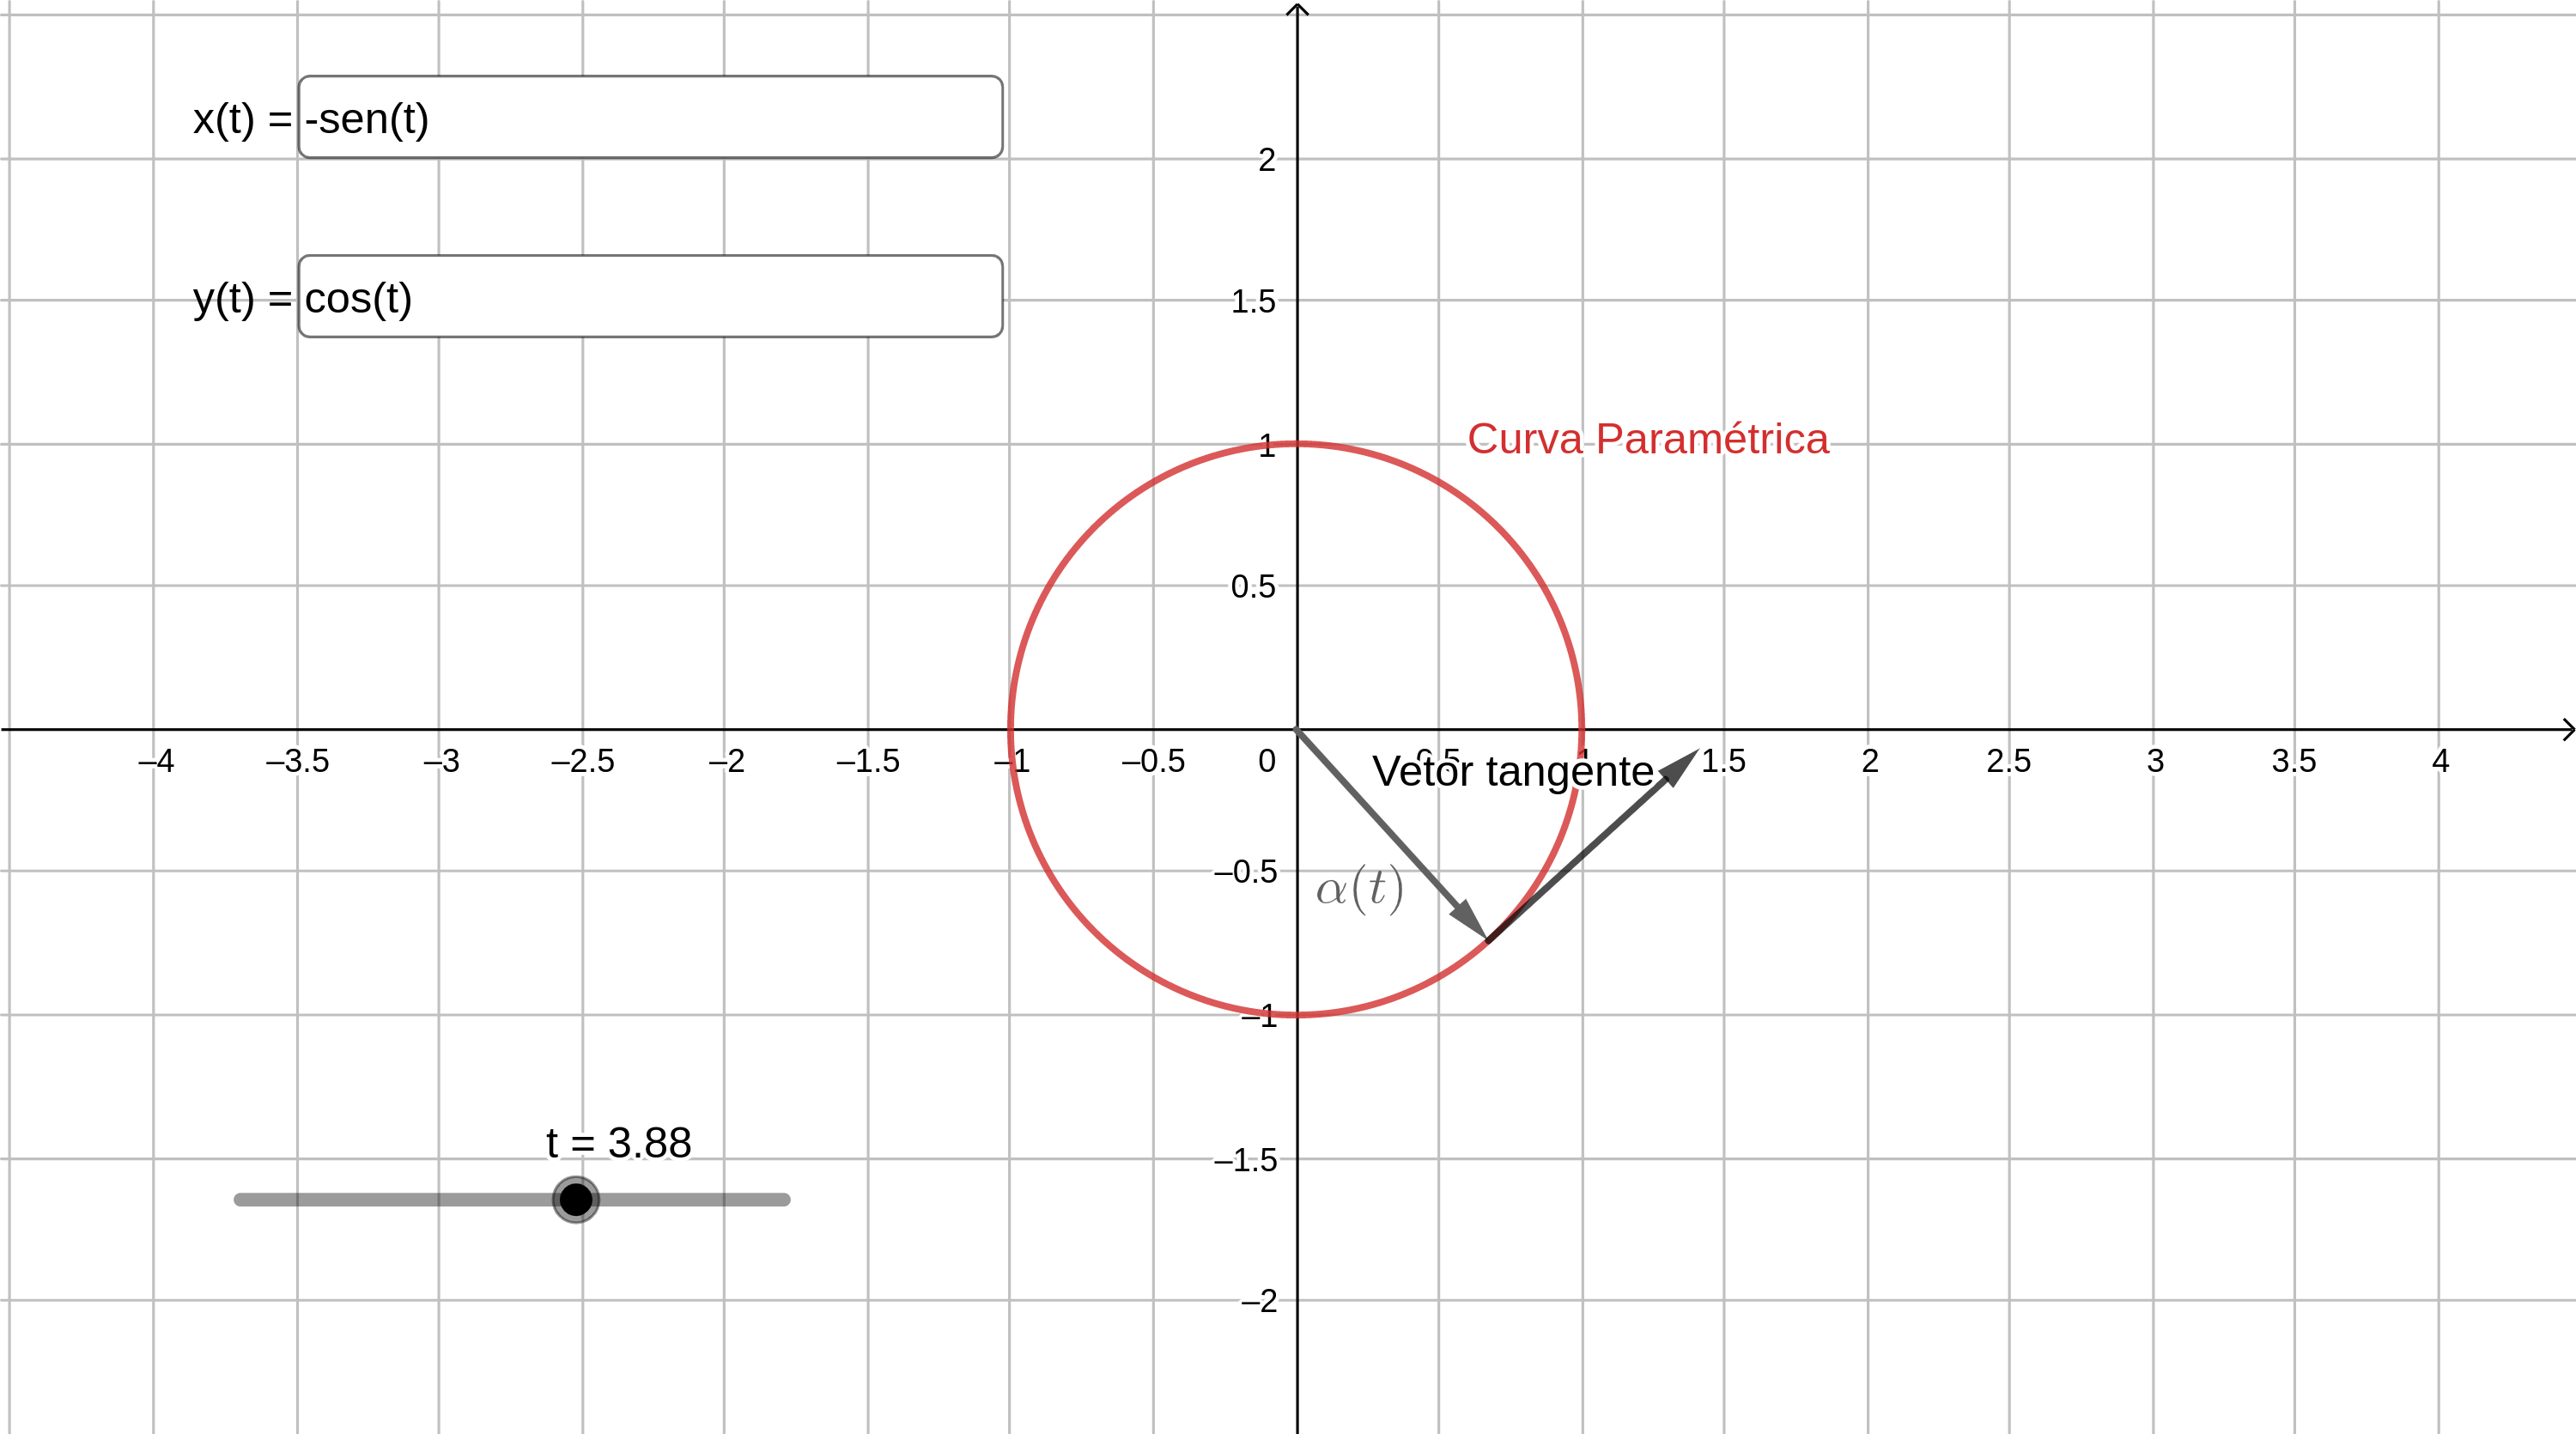
\includegraphics[width=\textwidth]{images/exe1.png}
        \caption{Snapshot de figura do exercício 1}
        \label{fig-exe1}
    \end{figure}

\end{solution}

\begin{exercise}
    Um {\it limaçon} (ou caracol de Pascal) é a curva parametrizada
    $$\gamma(t) = ((1 + 2\cos(t)).\cos(t); (1 + 2\cos(t)).\sin(t)), t \in \R.$$
    Faça o desenho desta curva. Observe que o ponto $(0, 0)$ pertence ao traço
    da curva, e ache o vetor tangente nesse ponto.
\end{exercise}

\begin{solution}

    Confira o desenho desta curva na Figura \ref{fig-exe2}.

    \begin{figure}[ht]
        \centering
        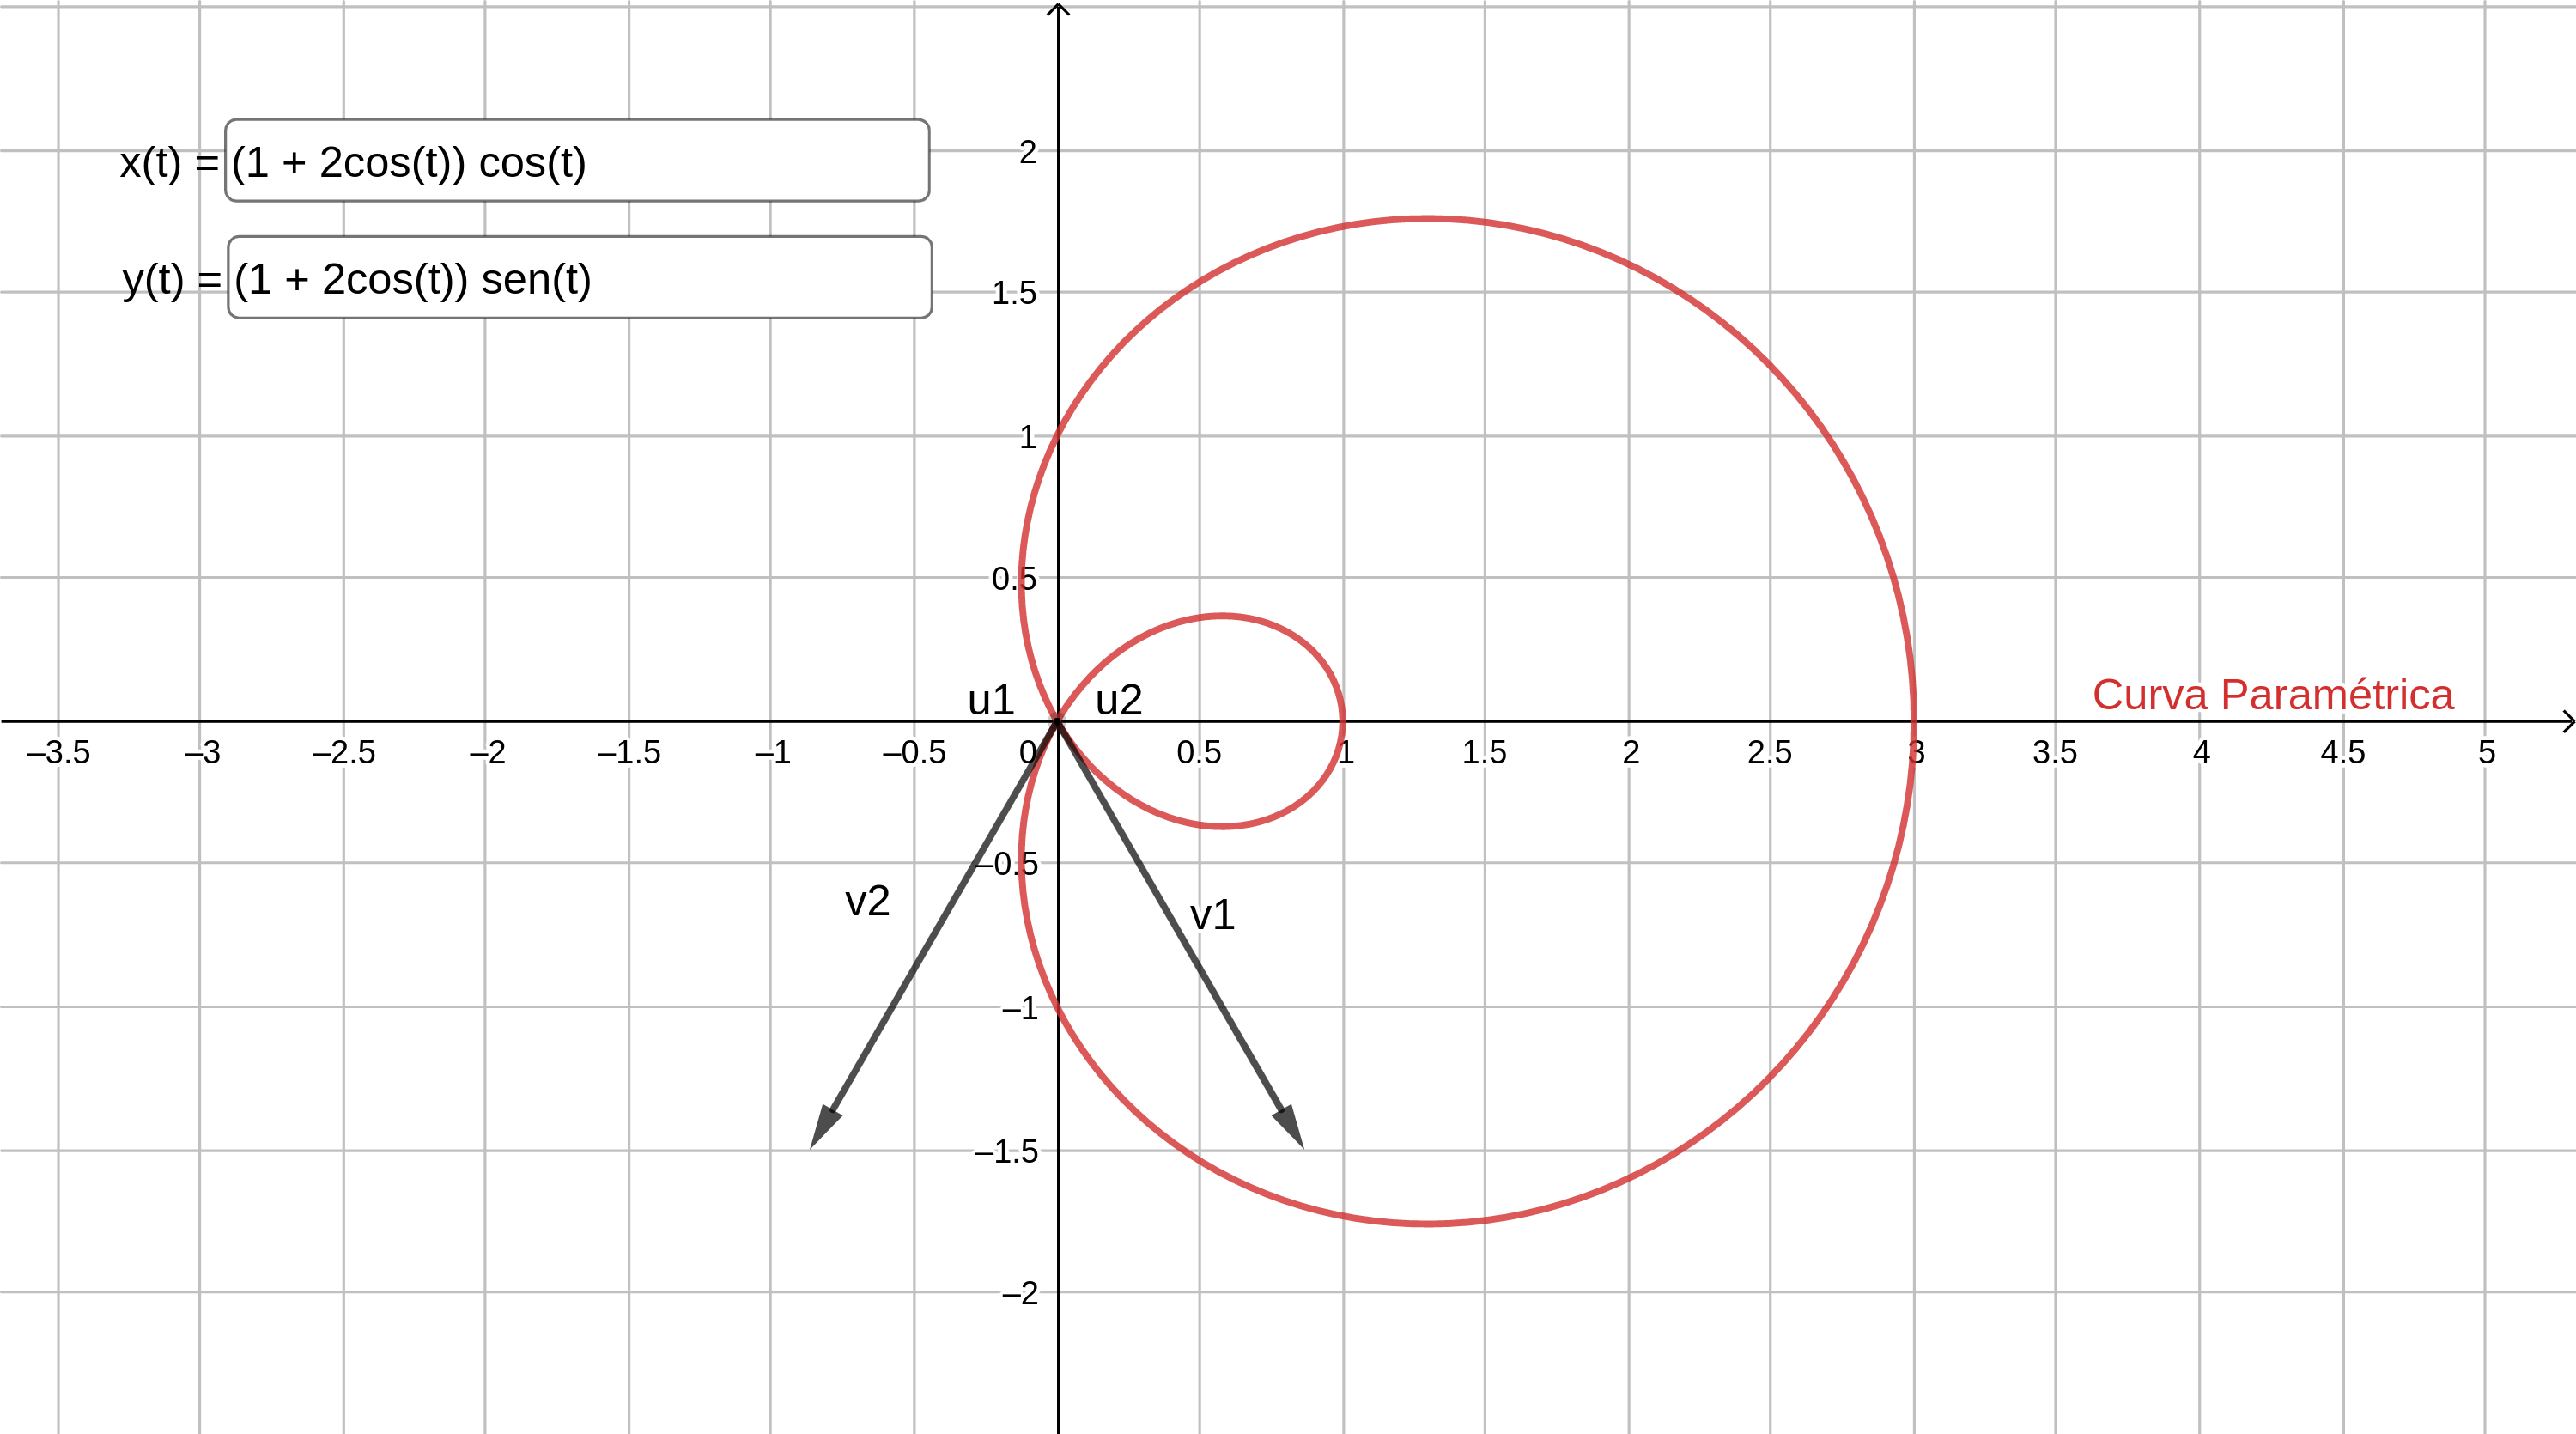
\includegraphics[width=\textwidth]{images/exe2.png}
        \caption{Snapshot de figura do exercício 2}
        \label{fig-exe2}
    \end{figure}

    De fato a curva passa pela origem se, e somente se, $\cos(t) = -1/2$. Em particular
    isso acontece quando $t = \frac{2}{3}\pi + 2\pi n$ ou $t = \frac{4}{3}\pi
    + 2\pi n$, onde $n \in \mathbb{Z}$. O vetor tangente dessa curva pode ser
    escrito como 
    \begin{equation*}
        \begin{split}
            \gamma '(t) &= (-(1 + 4\cos(t))\sin(t), \cos(t) + 2\cos^2(t) - 2\sin^2(t))  \\
            &= (-(1 + 4\cos(t))\sin(t), \cos(t) + 2\cos^2(t) - 2(1 - \cos^2(t))) \\
            &= (-(1 + 4\cos(t))\sin(t), \cos(t) + 4\cos^2(t) - 2)
        \end{split}        
    \end{equation*}
    Nos pontos considerados (quando $\cos(t) = -1/2$) temos
    $$
    \gamma(t^*) = (\sin(t^*), -1.5)
    $$
    Por fim, vamos ter dois vetores diferentes: 
    $$
    \gamma\left(\frac{2}{3}\pi\right) = \left(\frac{\sqrt{3}}{2}, -1.5\right) = v1
    $$
    $$
    \gamma\left(\frac{4}{3}\pi\right) = \left(-\frac{\sqrt{3}}{2}, -1.5\right) = v2
    $$
    Para mais detalhes, confira o arquivo Geogebra\footnote{\url{https://github.com/lucasmoschen/ta-sessions/blob/master/Curves_Surfaces/lists/list1/exercicio2.ggb}}
\end{solution}

\begin{exercise}
    A {\it Cissoide de Diocles} é a curva definida implicitamente pela equação
    $$x^3 + xy^2 - 2ay^2 
    = 0.$$
    Encontre uma parametrização para esta curva. Faça o desenho em Geogebra,
    incluindo a animação do vetor tangente percorrendo a curva. Busque
    informação para entender qual o fenômeno modelado por esta curva que a
    tornou famosa.
\end{exercise}

\begin{solution}
    Lembre que a cissoide de Diocles é o lugar geométrico da interseção da
    reta tangente a uma parábola com a reta perpendicular a ela que passa pela
    origem. Assim, esse ponto está em uma reta que passa pela origem. Em
    particular, podemos parametrizar de forma que $y = t\cdot x$ seja a
    equação desta reta e $t$ seja o parâmetro. Utilizando a equação, teremos 
    $$
    x^3 + x^3t^2 - 2ax^2t^2 = 0
    $$
    Se $x = 0$ essa igualdade é trivial. Mas caso não seja, dividindo ambos os
    lados por $x^2$ nos dá 
    $$
    x(1 + t^2) = 2at^2 \implies x = 2a\frac{t^2}{1 + t^2}
    $$
    Então uma parametrização para a cissoide é 
    $$
    \gamma(t) = 2a\frac{t^2}{1 + t^2}(1,t), t \in \mathbb{R}
    $$
    O desenho pode ser facilmente uma alteração nos arquivos dos exercícios 1
    ou 2, apenas mudando a função. Por isso, sugiro que olhe o arquivo que
    mostra a construção com a parábola da cissoide de
    Diocles\footnote{\url{https://github.com/lucasmoschen/ta-sessions/blob/master/Curves_Surfaces/lists/list1/exercicio3.ggb}}.
    
    Essa curva resolve o problema Delian: dada a aresta de um cubo, construir
    a aresta de um segundo cubo que tenha o volume do primeiro multiplicado
    por 2. Diocles usou para obter duas médias proporcionais a uma dada razão.
    
\end{solution}

\begin{exercise}
    O {\it Folium de Descartes} é definido implicitamente pela equação
    $$x^3 + y^3 = 3xy.$$ 
    Encontre uma parametrização para esta curva. Faça o desenho em Geogebra,
    incluindo a animação do vetor tangente percorrendo a curva. A descrição
    implícita desta curva da origem a uma familia de curvas da forma 
    $$F_{\epsilon}(x, y) = x^3 + y^3 - 3xy - \epsilon.$$
    Observe, usando o Geogebra, a mudança no traço da curva ao mudar de
    elemento da familia (ex.: $\epsilon = -\frac{1}{10}$)
\end{exercise}

\begin{solution}
    Uma ideia é procurar uma solução do tipo $y = xt$ novamente. Reescrevendo
    a equação, obtemos
    $$
    x^3 + x^3t^3 = 3x^2t
    $$
    Se $x=0$, a equação é trivialmente satisfeita. Agora suponha $x \neq 0$ e
    obtemos 
    $$
    x(1 + t^3) = 3t \implies x(t) = \frac{3t}{1 + t^3}
    $$
    Um primeiro problema que aparece nessas contas é que pedimos para $t \neq
    -1$. Todavia, para representar a curva, precisamos que $t \in \R-\{-1\}$,
    que não é um intervalo. Por esse motivo, algumas referências definem uma
    {\bf representação legal} de um arco como uma aplicação contínua em um intervalo e uma curva é a
    união de representações legais de arco. Confira o livro {\it A Catalog of
    Special Plane Curves} de Dennis Lawrence. 
    
    Portanto concluímos que a parametrização é dada por 
    $$
    \alpha(t) = \frac{3t}{1 + t^3}(1, t), \text{ tal que } t \in \R - \{-1\}
    $$
    O curioso de desenhar o vetor tangente é que a maior parte da curva é
    feita próximo ao valor de -1. Mas você pode conferir o arquivo Geogebra no
    Github \footnote{\url{https://github.com/lucasmoschen/ta-sessions/blob/master/Curves_Surfaces/lists/list1/exercicio4.ggb}}.

    \begin{figure}[ht]
        \centering
        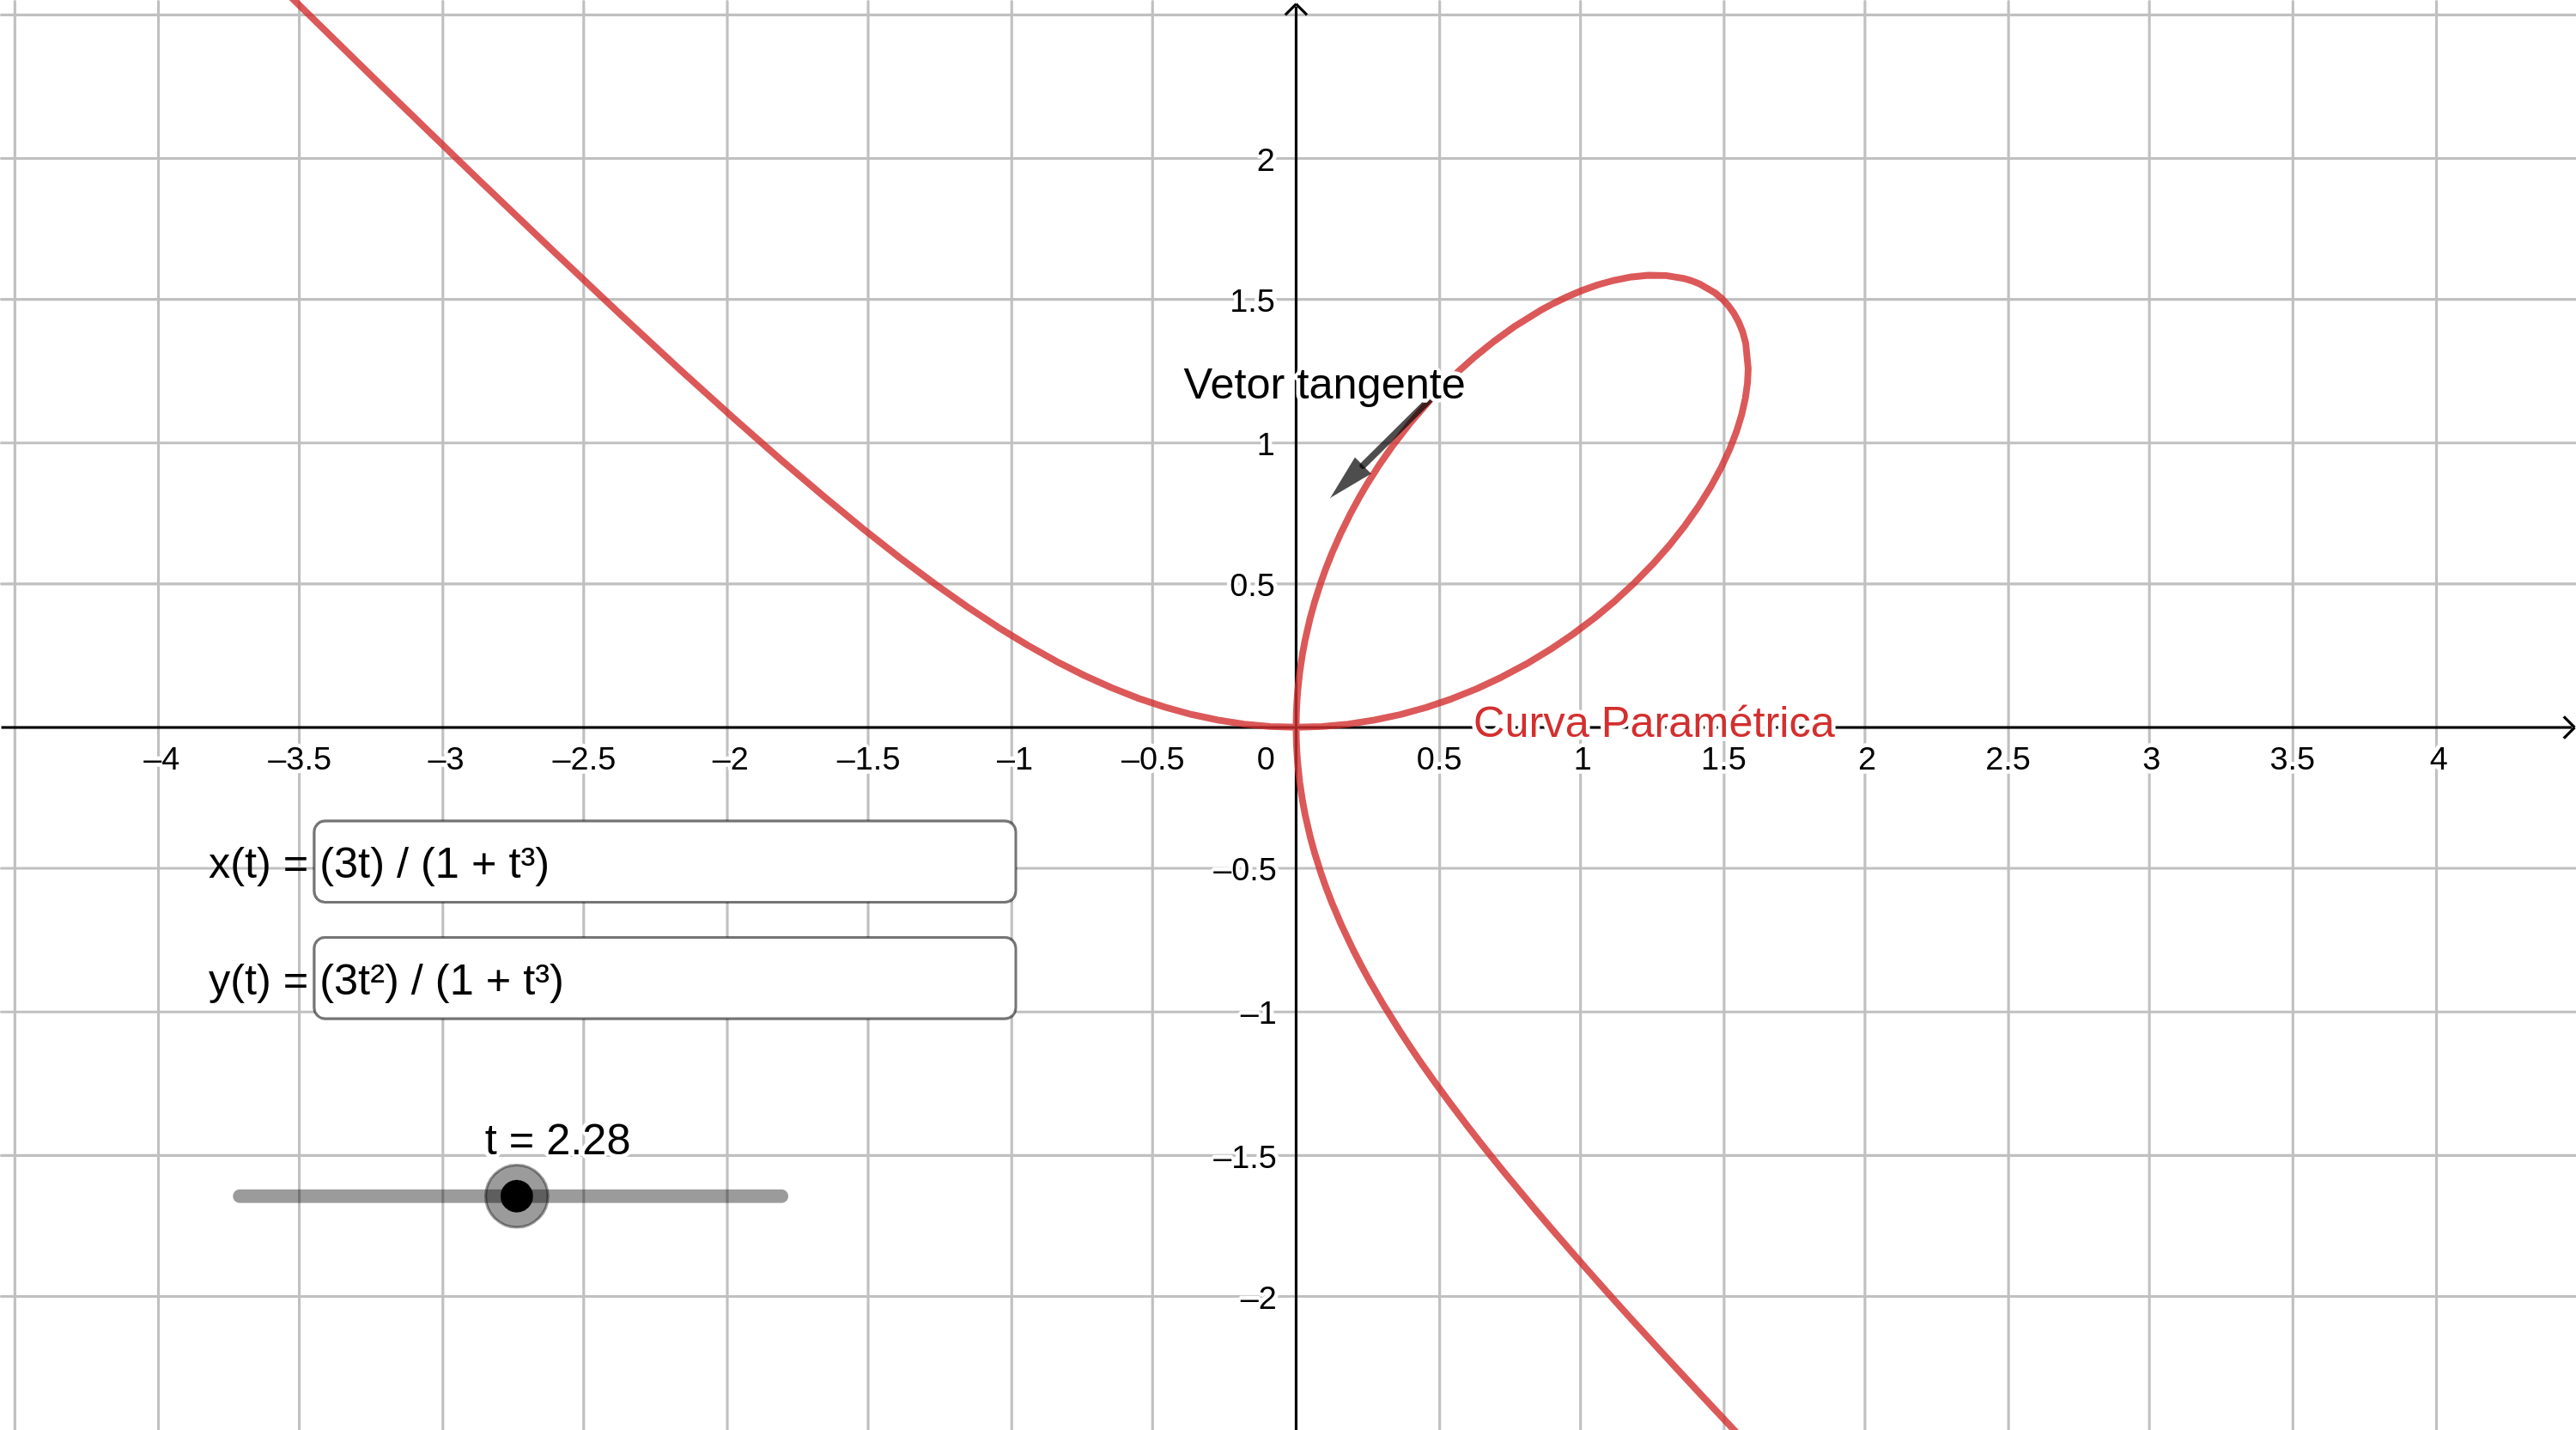
\includegraphics[width=\textwidth]{images/exe4.png}
        \caption{Snapshot de figura do exercício 4}
        \label{fig-exe4}
    \end{figure}
    
    Dê uma olhada no arquivo \texttt{images/foliumeps.gif} na mesma pasta do
    arquivo {\tt .ggb}. 

\end{solution}


\begin{exercise}
    Verifique que a aplicação $\alpha(t) = (a\cos(t), b\sin(t)), t \in \R$, com $a$ e $b$ constantes não-nulas, é uma curva parametrizada diferenciável. Descreva o traço de $\alpha$.
\end{exercise}

\begin{solution}
    Seja $\beta(t) = (-a\sin(t), b\cos(t))$. Vou provar que 
    $$
    \lim_{h\to 0} \frac{\alpha(t+h) - \alpha(t) -  h\beta(t)}{|h|} = 0 
    $$
    Ou seja,
    $$
    \lim_{h\to 0} \frac{(a(\cos(t + h) - \cos(t) + h\sin(t)), b(\sin(t+h) - \sin(t) - h\cos(t))}{|h|} = (0,0) 
    $$ 
    Dado que as funções cosseno e seno são diferenciáveis, podemos utilizar
    polinômios de Taylor para obter
    $$
    \cos(t + h) - \cos(t) + h\sin(t) = -h\sin(t) + o(h) + h\sin(t) = o(h)
    $$
    $$
    \sin(t+h) - \sin(t) - h\cos(t) = h\cos(t) + o(h) - h\cos(t) = o(h)
    $$

    Portanto basta calcularmos $\lim_{h\to 0}\frac{(o(h),
    o(h))}{|h|}$ que é $(0,0)$ por definição. Essa notação é chamada de {\it
    little o-notation} e é muito importante nesse tipo de estudo.\footnote{\url{https://en.wikipedia.org/wiki/Big_O_notation\#Little-o_notation}}

    Observe que $\left(\frac{x(t)}{a}\right)^2 + \left(\frac{y(t)}{b}\right)^2
    = \cos(t)^2 + \sin(t)^2 = 1$, logo o traço dessa curva é uma elipse. 
\end{solution}

\begin{exercise}
    Obtenha uma curva regular $\alpha : \R \to \R^2$ tal que $\alpha(0) = (2, 0)$ e $\alpha'(t) = (t^2 , e^t )$.    
\end{exercise}

\begin{solution}
    A regularidade da curva vem de que $e^t \neq 0, \forall t \in R$. Pelo
    Teorema Fundamental do Cálculo, 
    $$
    \alpha(t) = \int_0^t \alpha '(s) ds + C = \int_0^t (s^2, e^s)ds + C = \left(\frac{t^3}{3}, e^t - 1\right) + C, 
    $$
    tal que $(2, 0) = \alpha(0) = (0, 0) + C \implies C = (2,0)$ e, portanto, 
    $$
    \alpha(t) = (t^3/3 + 2, e^t - 1)
    $$
\end{solution}

\begin{exercise}
    Seja $\alpha : I \to \R^2$ uma curva regular. Prove que $$||\alpha'(t)||$$ é constante se, e somente se,
    para cada $t \in I$, o vetor $\alpha ''(t)$ é ortogonal a $\alpha '(t)$.    
\end{exercise}

\begin{solution}
    Suponha inicialmente que $\beta(t) = ||\alpha '(t)||^2 = \langle \alpha'(t), \alpha
    '(t) \rangle$ é constante. Portanto, 
    $$
    \beta'(t) = 2\langle a'(t), a''(t) \rangle = 0 \implies \alpha'(t) \perp \alpha''(t)
    $$
    Agora suponha que $\alpha'(t) \perp \alpha''(t)$. Então 
    $$
    0 = 2\langle a'(t), a''(t) \rangle = \beta'(t)
    $$
    o que implica $\beta(t)^{1/2} = ||\alpha '(t)||$ ser constante.  


    \begin{remark}[Derivação de produto interno]
        \url{https://math.stackexchange.com/questions/96265/differentiating-an-inner-product}.
        Como $\alpha': I \to \R^2$, podemos escrever $\langle a'(t), a'(t)
        \rangle = x'(t)^2 + y'(t)^2$ onde $x$ e $y$ são coordenadas funções de
        $t$. Nesse caso 
        $$
        \frac{d}{dt}(x'(t)^2 + y'(t)^2) = 2x'(t)x''(t) + 2y'(t)y''(t) = 2\langle \alpha '(t), \alpha''(t) \rangle
        $$
    \end{remark}
\end{solution}

\begin{exercise}
    Prove que, se uma curva regular $\alpha(t) = (x(t), y(t)), t \in I \subset
    \R$, é tal que $x'(t) \neq 0, \forall t \in I$, então o traço de $\alpha$ é o gráfico de uma função diferenciável.
\end{exercise}

\begin{solution}
    Vamos provar que para qualquer $x \in x(I)$, onde $x(I) = \{x | (x(t),
    y(t)) \in \alpha(I) \text{ e } x(t) = x\}$, existe um único $y$ associado
    a ele na curva $\alpha$. Para isso tome dois pontos quaisquer diferentes na curva
    $(x(t_1), y(t_1))$ e $(x(t_2), y(t_2))$, tal que $t_1 > t_2$, sem perda de
    generalidade. Pelo teorema do valor médio 
    $$
    x(t_1) - x(t_2) = x'(\xi)(t_1 - t_2) \neq 0,  \xi \in (t_1, t_2)
    $$
    Portanto para quaisquer pontos $t_1 > t_2$, teremos que $x(t_1) \neq
    x(t_2)$. Como na curva não existem dois pontos com a mesma coordenada $x$,
    podemos associar uma função $f: x(I) \to y(I)$ definida de forma que 
    $f(x) = y$ se $(x,y) \in \alpha(I)$. Falta provar que $f$ é diferenciável.
    Tome $x$ no interior de $x(I)$ e $h$ suficientemente pequeno de forma que
    $x + h \in x(I)$. Suponha que $x+h = x(t_2)$ e $x = x(t_1)$. Assim:
    $$
    \lim_{h \to 0} \frac{f(x + h) - f(x)}{x + h - x} = \lim_{h\to 0}\frac{y(t_2) - y(t_1)}{x(t_2) - x(t_1)} = \lim_{h\to 0} \frac{\frac{y(t_2) - y(t_1)}{t_2 - t_1}}{\frac{x(t_2) - x(t_1)}{t_2-t_1}}
    $$
    
    Provamos que a função $x(t)$ é injetiva em $I$. Em particular $x: I \to
    x(I)$ é bijetiva e admite inversa. Como $x$ é contínua sua inversa também
    é contínua\footnote{Uma prova para isso pode ser conferida nesse texto
    \url{https://www.maths.tcd.ie/~richardt/121/121-ch4.pdf}}. Isso serve para
    mostrar que como $h \to 0$, então $t_2 \to t_1$ e, portanto, $f'(x) =
    y'(t_1)/x'(t_1)$, o que prova que $f$ é derivável. 
    

\end{solution}

\begin{exercise}
    Considere a espiral logarítmica $\gamma : \R \to \R^2$ definida por
    $\gamma(t) = (e^t\cdot\cos(t), e^t\cdot\sin(t))$. Desenhe a curva em
    ambiente computacional e mostre que o ângulo entre $\gamma(t)$ e o vetor tangente em $\gamma(t)$ não depende de $t$.
\end{exercise}

\begin{solution}
    Primeiro vamos provar que o ângulo não depende de $t$. Temos que $\gamma
    '(t) = (e^t(\cos(t) - \sin(t)), e^t(\sin(t) + \cos(t)))$. Seja $\theta(t)$
    esse ângulo, então
    $$
    \cos(\theta(t)) = \frac{\langle \gamma(t), \gamma '(t) \rangle}{||\gamma(t)||||\gamma '(t)||} = \frac{e^{2t}(\cos^2(t) - \cos(t)\sin(t) + \sin^2(t) + \sin(t)\cos(t))}{\sqrt{2}e^{2t}} = \frac{1}{\sqrt{2}}
    $$

    Como o ângulo entre dois vetores é nunca maior do que $\pi$, então podemos
    inverter o cosseno e termos $\theta(t)$ constante. 

    Confira no Github a animação da
    curva\footnote{\url{https://github.com/lucasmoschen/ta-sessions/blob/master/Curves_Surfaces/lists/list1/exercicio9.ggb}}.
    Observe que existe erro de cálculo na maneira que eu encontrei o ângulo,
    existem formas mais matemáticas para evitar erro numérico, mas não é
    necessário nesse caso. 

\end{solution}

\end{document}